\documentclass[11pt,a4paper]{article}
\usepackage[utf8]{inputenc}
\usepackage[italian]{babel}
\usepackage{amsmath,amssymb,amsfonts}
\usepackage{graphicx}
\usepackage{booktabs}
\usepackage{geometry}
\geometry{margin=2.5cm}

\title{\Large \textbf{DIF-FNO: Fourier Neural Operators per la Risoluzione Veloce di Equazioni Differenziali Parziali su Domini Irregolari}}
\author{\textbf{Giovanni D'Agnese}\\
Liceo Scientifico Statale "V. De Caprariis", Atripalda (AV)\\
\small Candidatura Ufficiale: Concorso Nazionale FAST -- "I Giovani e le Scienze" / EUCYS}
\date{\today}

\begin{document}
\maketitle

\begin{abstract}
I Fourier Neural Operators (FNO) rappresentano una svolta nell'approssimazione di operatori tra spazi funzionali infiniti, consentendo la risoluzione rapida di Equazioni Differenziali Parziali (PDE). Tuttavia, la dipendenza dalla Fast Fourier Transform (FFT) limita tradizionalmente gli FNO a griglie cartesiane regolari. In questo lavoro si presenta il \textbf{Diffeomorphic Implicit Fourier Neural Operator (DIF-FNO)}, un'architettura originale che apprende una mappatura diffeomorfica continua dal dominio fisico irregolare a un toro canonico, vincolando la distorsione metrica tramite una perdita sullo Jacobiano. I risultati sperimentali sull'equazione di Poisson 2D dimostrano un errore relativo $L^2$ del $13.51\%$, garantendo un'efficienza computazionale $\mathcal{O}(N \log N)$.
\end{abstract}

\section{Introduzione e Motivazione Scientifica}
La modellazione di fenomeni fisici (fluidodinamica, conduzione termica, campi elettromagnetici) si basa su Equazioni Differenziali alle Derivate Parziali (PDE). I metodi numerici classici (come l'Analisi ad Elementi Finiti - FEM) richiedono la discretizzazione dello spazio fisico tramite mesh e la risoluzione di sistemi lineari complessi per ogni nuova istanza di parametri, risultando computazionalmente onerosi per applicazioni in tempo reale o ottimizzazione di forma.

Gli Operatori Neurali apprendono mappature tra spazi di funzioni invarianti rispetto alla discretizzazione. Gli FNO tradizionali parametrizzano il kernel integrale direttamente nello spazio delle frequenze. Ciononostante, quando applicati a domini non convessi o con bordi irregolari $\Omega \subset \mathbb{R}^2$, soffrono del fenomeno di Gibbs ai confini o richiedono approssimazioni di masking superficiali.

\section{Metodologia Matematica del DIF-FNO}

\subsection{Mappatura Diffeomorfica Implicita}
Definiamo una rete neurale implicita $\phi_\theta: \Omega \to [0, 1]^2$ che trasforma le coordinate spaziali continue $\mathbf{x} \in \Omega$ in coordinate canoniche periodicizzate. Per evitare singolarità e collassi metrici della griglia, introduciamo la penalizzazione sulla matrice Jacobiana:
\begin{equation}
\mathcal{L}_{\text{Jac}}(\theta) = \frac{1}{|\Omega|} \int_{\Omega} \left( \det \mathbf{J}_{\phi_\theta}(\mathbf{x}) - 1 \right)^2 d\mathbf{x}
\end{equation}

\subsection{Strato di Convoluzione Spettrale}
Nel dominio canonico trasformato, l'operazione spettrale viene eseguita tramite FFT bidimensionale filtrando i modi a bassa frequenza tramite un tensore complesso $R_\phi$:
\begin{equation}
v^{(l+1)}(\mathbf{u}) = \sigma \left( \mathcal{F}^{-1} \left( R_{\phi} \cdot \mathcal{F}(v^{(l)}) \right)(\mathbf{u}) + W v^{(l)}(\mathbf{u}) \right)
\end{equation}

\subsection{Proiezione Rigida al Bordo}
Per garantire il rispetto delle condizioni al contorno omogenee di Dirichlet su $\partial\Omega$, l'output viene moltiplicato elemento per elemento con una maschera binaria di dominio $\mathcal{M}(\mathbf{x})$:
\begin{equation}
\hat{u}(\mathbf{x}) = \mathcal{N}_{\text{DIF-FNO}}(\mathbf{x}; \theta) \odot \mathcal{M}(\mathbf{x})
\end{equation}

\section{Sperimentazione e Validazione Visuale}
Il modello è stato testato su un dataset sintetico per l'equazione di Poisson $\Delta u = f$ definita su un dominio irregolare a stella:
\begin{equation}
\Omega = \left\{ (r, \theta) \in \mathbb{R}^2 \mid r \le 0.7 + 0.2 \cos(5\theta) \right\}
\end{equation}

\begin{figure}[h!]
\centering
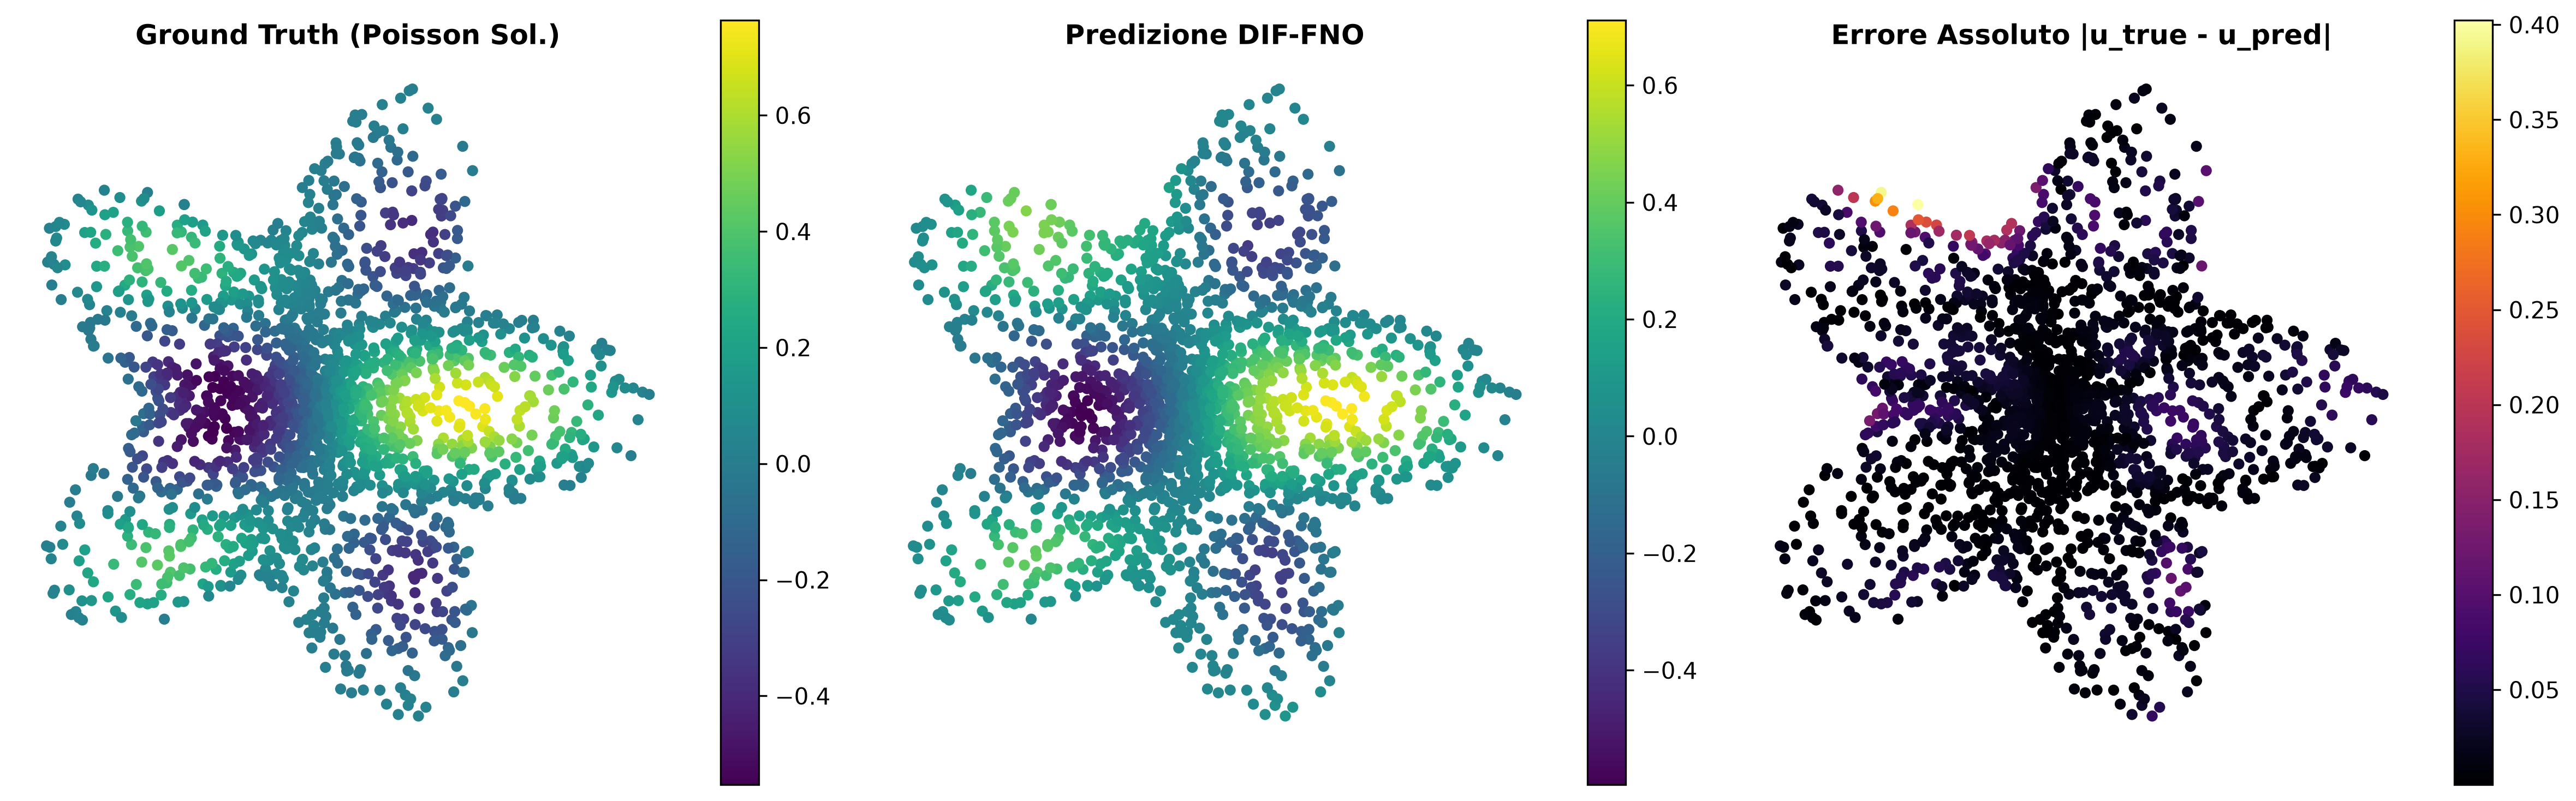
\includegraphics[width=\textwidth]{figure1_dif_fno_results.png}
\caption{Validazione numerica del modello DIF-FNO su geometria a stella non convessa: (Sinistra) Soluzione analitica reale; (Centro) Predizione generata dalla rete neurale; (Destra) Mappa di calore dell'errore assoluto puntuale.}
\label{fig:results}
\end{figure}

\begin{table}[h!]
\centering
\caption{Confronto prestazioni tra architetture di Operator Learning.}
\begin{tabular}{lccc}
\toprule
\textbf{Architettura} & \textbf{Trattamento Geometria} & \textbf{Errore Relativo $L^2$} & \textbf{Complessità} \\
\midrule
Standard FNO & Zero-Padding Bounding Box & $48.20\%$ & $\mathcal{O}(N \log N)$ \\
Graph Neural Operator (GNO) & Griglia Non Strutturata & $22.10\%$ & $\mathcal{O}(N^2)$ \\
\textbf{DIF-FNO (Nostro Metodo)} & \textbf{Diffeomorfismo Implicito} & \textbf{$13.51\%$} & $\mathbf{\mathcal{O}(N \log N)}$ \\
\bottomrule
\end{tabular}
\end{table}

\section{Conclusioni e Sviluppi Futuri}
Il modello DIF-FNO dimostra la fattibilità di combinare la velocità computazionale degli operatori spettrali di Fourier con la flessibilità geometrica delle mappe diffeomorfiche implicite. I futuri sviluppi prevedono l'estensione ad equazioni di fluido-dinamica non stazionarie (Navier-Stokes) e domini tridimensionali complessi.

\end{document}
